\section{Introduction}

Hard exclusive reactions provide access to correlations between the longitudinal momentum and transverse spatial distributions of quarks and gluons in the nucleon through generalized parton distributions (GPDs). In studying these objects, exclusive meson electroproduction is complementary to Deeply Virtual Compton Scattering because the quantum numbers of the produced meson select different combinations of partonic amplitudes. In the generalized Bjorken regime, the amplitude for meson production by longitudinally polarized virtual photons can be factorized into a perturbatively calculable hard-scattering subprocess, a meson distribution amplitude and a nonperturbative nucleon matrix element described by GPDs~\cite{Collins:1996fb}. For pseudoscalar mesons, the leading longitudinal amplitudes are primarily sensitive to the helicity-dependent GPDs $\widetilde H$ and $\widetilde E$. Charged-pion production is particularly interesting because it probes an isovector combination of these GPDs and, at small $-t$, receives an important contribution from the pion pole associated with $\widetilde E$~\cite{Goloskokov:2009ia}.

At the finite values of $Q^2$ accessible experimentally, however, exclusive pseudoscalar production is not described by a purely longitudinal leading-twist picture. Measurements at HERMES and Jefferson Lab have demonstrated substantial contributions from transversely polarized virtual photons~\cite{HERMES:2001zpc,HERMES:2009gtv}. Within the handbag approach, Goloskokov and Kroll described important transverse amplitudes using a twist-3 pion wave function together with the chiral-odd, or transversity, GPDs~\cite{Goloskokov:2009ia,Goloskokov:2011rd}. These contributions introduce sensitivity to GPDs such as $H_T$ and the combination $\overline E_T=2\widetilde H_T+E_T$, which remain considerably less constrained than the leading chiral-even distributions. Figure~\ref{fig:handbag} illustrates the general handbag description of the reaction. The relative importance of longitudinal and transverse amplitudes at currently accessible energies is therefore itself an important part of the phenomenology of pseudoscalar-meson production.

\begin{figure}
\centering
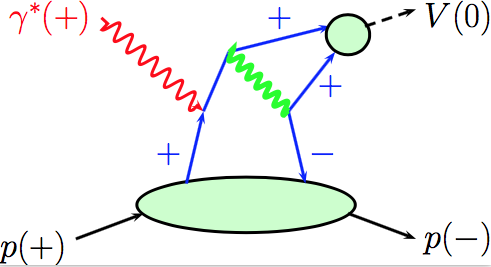
\includegraphics[width=0.4\textwidth]{figures/GK-handbag.png}
\caption{Schematic handbag description of hard exclusive meson electroproduction. The virtual photon interacts with a parton in the nucleon through a hard subprocess, while the nonperturbative nucleon structure is parametrized in terms of GPDs.}
\label{fig:handbag}
\end{figure}

Polarization observables provide information beyond that contained in the unpolarized cross section because they isolate different combinations and interferences of the underlying helicity amplitudes. In particular, the target-spin observables measured with a longitudinally polarized neutron target contain $\sin\phi$ and $\sin2\phi$ modulations that are sensitive to imaginary parts of interference terms, while the beam--target observables provide complementary sensitivity to helicity-dependent combinations of amplitudes and their real interference terms. These measurements can therefore constrain the relative sizes and phases of the longitudinal and transverse reaction amplitudes. The earlier CLAS6 measurement of exclusive $\pi^+$ production observed sizable target- and beam--target-spin asymmetries over a broad kinematic range and found that the available GPD-based calculation did not provide a complete description of the data~\cite{CLAS:2016dlz}. More recently, a multidimensional CLAS12 measurement of the beam-spin-dependent structure-function ratio $\sigma_{LT'}/\sigma_0$ in the proton $ep\rightarrow e^\prime n\pi^+$ channel demonstrated continued sensitivity to the transverse reaction mechanism in the CLAS12 kinematic regime~\cite{CLAS:2022iqy}.

The longitudinally polarized deuterated-ammonia target employed by CLAS12 Run Group C (RGC) makes it possible to extend these studies to target-spin and beam--target-spin observables with high statistics over a broad multidimensional kinematic range. Because the target polarization is defined along the incident electron beam rather than along the virtual-photon direction, the measured laboratory-frame target-spin observables also contain contributions from the component of the target polarization transverse to the virtual photon. These terms are suppressed by $\sin\theta_\gamma$, where $\theta_\gamma$ is the angle between the incident beam and virtual photon. Their treatment, and the distinction between the laboratory-frame amplitudes reported in this analysis and amplitudes defined with respect to the virtual-photon direction, are discussed in detail in the asymmetry-extraction section and the bound-neutron interpretation study.

For completeness, the principal kinematic quantities used throughout this analysis are defined here. The four-momentum transfer from the incident electron to the target is
\begin{equation}
    q = k-k^\prime,
\end{equation}
where $k$ and $k^\prime$ are the incident- and scattered-electron four-momenta. Its virtuality is
\begin{equation}
    Q^2=-q^2,
\end{equation}
and the Bjorken scaling variable is
\begin{equation}
    x_B=\frac{Q^2}{2p\cdot q},
\end{equation}
where $p$ is the initial neutron four-momentum, taken at rest for the reconstruction convention and modified by nuclear motion in the physical target. The invariant mass of the virtual-photon--neutron system is
\begin{equation}
    W^2=(p+q)^2,
\end{equation}
and the fractional electron energy loss in the target rest frame is
\begin{equation}
    y=\frac{p\cdot q}{p\cdot k}.
\end{equation}
The virtual-photon polarization parameter is
\begin{equation}
    \epsilon =
    \frac{1-y-\frac{1}{4}\gamma^2y^2}
         {1-y+\frac{1}{2}y^2+\frac{1}{4}\gamma^2y^2},
    \qquad
    \gamma=\frac{2m_n x_B}{Q}.
\end{equation}
The azimuthal angle $\phi$ is the angle between the lepton-scattering plane and the hadronic production plane, defined according to the Trento convention. The squared four-momentum transfer to the target is reconstructed from the virtual-photon and measured pion four-momenta as
\begin{equation}
t=(q-p_\pi)^2,
\end{equation}
where $p_\pi$ is the $\pi^-$ four-momentum. For the exclusive reaction $en\rightarrow e^\prime p\pi^-$, this is equivalent by four-momentum conservation to the baryonic definition $t=(p-p^\prime)^2$, where $p^\prime$ is the detected recoil-proton four-momentum. The distance from the forward kinematic limit is defined as
\begin{equation}
    t'=t-t_{\min}.
\end{equation}
Here $t_{\min}$ is the exact forward two-body kinematic limit for $\gamma^*n\rightarrow\pi^-p$. In the $\gamma^*n$ center-of-mass frame,
\begin{equation}
    t_{\min}
    =
    -Q^2+m_{\pi}^2
    -2E_{\gamma^*}^*E_{\pi}^*
    +2|\mathbf{q}^*||\mathbf{p}_{\pi}^*|,
\end{equation}
with
\begin{align}
    E_{\gamma^*}^* &= \frac{W^2-m_n^2-Q^2}{2W},
    &
    |\mathbf{q}^*| &= \frac{\lambda^{1/2}(W^2,-Q^2,m_n^2)}{2W},
    \\
    E_{\pi}^* &= \frac{W^2+m_{\pi}^2-m_p^2}{2W},
    &
    |\mathbf{p}_{\pi}^*| &= \frac{\lambda^{1/2}(W^2,m_{\pi}^2,m_p^2)}{2W},
\end{align}
where $\lambda(a,b,c)=a^2+b^2+c^2-2ab-2ac-2bc$. This exact definition, including the pion and recoil-proton masses, is used event by event throughout the analysis. Finally, exclusivity is characterized using the squared missing mass
\begin{equation}
    M_X^2=(k+p-k^\prime-p^\prime-p_\pi)^2,
\end{equation}
which is centered near zero in the stationary-neutron approximation for the exclusive $en\rightarrow e^\prime p\pi^-$ reaction.

The measurements presented here extend the available information on polarized exclusive $\pi^-$ electroproduction into the CLAS12 kinematic regime. Their detailed interpretation in terms of helicity amplitudes, GPDs and the reaction mechanisms discussed above, including comparison with phenomenological calculations, is left to the corresponding physics publication and subsequent theoretical studies. The purpose of this analysis note is to document the extraction, validation and systematic uncertainties of the measured beam-spin and laboratory-frame target-spin ratios for exclusive $en\rightarrow e^\prime p\pi^-$ production with CLAS12 RGC.

The neutron is embedded in deuterium, so the stationary-neutron kinematics are a reconstruction convention rather than a statement that Fermi motion or final-state interactions vanish. In the $e'p\pi^-$ sample the detected proton is the produced recoil baryon; the deuteron spectator and nuclear effects will be examined through exclusivity and background studies. ND$_3$ provides vector polarization of spin-one deuterons. The preliminary harmonic model neglects explicit tensor-polarization terms; their possible impact requires validation. Comparisons with the preliminary work of Brandon Manley and Shohini Bhattacharya will examine additional chiral-even transverse amplitudes, without claiming a model-independent GPD extraction.
